\documentclass[
	%parspace, % Add vertical space between paragraphs
	%noindent, % No indentation of first lines in each paragraph
	%nohyp, % No hyphenation of words
	twoside % Double sided format
	%draft, % Quicker draft compilation without rendering images
	%final, % Set final to hide todos
]{elteikthesis}[2024/04/26]
\title{Comparison of edge detection methods}
\date{2025}
\author{Petrányi Bálint}
\degree{Computer Science BSc}
\supervisor{Gede Mátyás}
\affiliation{Associate Professor}
\university{Eötvös Loránd University}
\faculty{Faculty of Informatics}
\department{Institute of Cartography and Geoinformatics}
\city{Budapest}
\logo{elte_cimer_szines}

\usepackage{acronym}
\usepackage{pgfplotstable}
\usepackage{pgfplots}

\newcommand{\CC}{C\nolinebreak\hspace{-.05em}\raisebox{.4ex}{\tiny\bf +}\nolinebreak\hspace{-.10em}\raisebox{.4ex}{\tiny\bf +}}
\def\CC{{C\nolinebreak[4]\hspace{-.05em}\raisebox{.4ex}{\tiny\bf ++}}}

\newcommand{\GG}{G\nolinebreak\hspace{-.05em}\raisebox{.4ex}{\tiny\bf +}\nolinebreak\hspace{-.10em}\raisebox{.4ex}{\tiny\bf +}}
\def\GG{{G\nolinebreak[4]\hspace{-.05em}\raisebox{.4ex}{\tiny\bf ++}}}

\addbibresource{thesis.bib}

\begin{document}
\documentlang{english}

\maketitle

\tableofcontents
\cleardoublepage

\chapter{Introduction}
\label{chap:intro}

The aim of this thesis is to show the differences of edge detectors and the difference of two main \ac{GPGPU} programming libraries namely OpenCl and Cuda.

This thesis topic is mainly aims to answer the question of what \ac{GPGPU} library is the better and exactly how important it is to do graphics and/or computer vision related tasks on the \ac{GPU}. While we know by the structure of how these libraries operate that Cuda will be the most optimal of the two, we cannot be sure of this before testing this out.

The reason I chose this topic is because while I was studying \ac{GPGPU} during my university years I discovered that there's little evidence proving that Cuda is faster. While there are many discussions online suggesting Cuda is faster, there have been no research or tests done on this topic, thus I decided to test it myself. I chose edge detection as the test because they are easy to understand and the algorithms for them are already optimized. I use two edge detection algorithms. One is by far one of the most used \ac{Canny}. The other algorithm is the \ac{DoG} which is a far more simple algorithm than \ac{Canny} and it should finish a lot faster.

This thesis is organised into four chapters. The first chapter is this one which serves as an introduction to the topic and goals of this thesis.

The second chapter is the user documentation. It introduces the program to an end user. Demonstrating how to install, what are the requirements for running and example usages.

The third chapter is a developer documentation explaining how the code works, what tests were conducted, what was my plan going into development, what technologies I used, and generally the inner workings of the program.

The forth and final chapter will be a summary of my findings during the thesis. I will review what should be expected if the tests are conducted on different machines and methods to optimize the code better and what other edge detectors I could implement.
\cleardoublepage
\chapter{User Documentation}

In this chapter we will explore the usage of the program from the perspective of and end user. We define the minimum requirements for the programs running, provide ways for installation and show example usages of the program.

\section{Program requirements}

The program can run on any 64 bit processor and is prepared to run on Windows and Linux operating system. The program can run with only a \ac{CPU} but for it to work with OpenGl it needs a \ac{GPU} that is capable to run atleast 1024 concurrent threads. The CUDA functionality requires an NVIDIA \ac{GPU} whit the same concurrent thread requirement.

\section{Installation guide}

The program requires no installation for an end user. You only need to download the provided compressed binaries for your operating system from the following website \hyperref{https://github.com/Palnit/BSC-Thesis}{https://github.com/Palnit/BSC-Thesis} and unzip the binary and run. If you want to build it for your self with CUDA capability you need to download the CUDA SDK from \hyperref{test}{test} and CMAKE with a cpp build system e.g.: ninja, make and a compiler e.g.: g++, MSVC, Clangd. 




\cleardoublepage
\chapter{Developer Documentation}

In this chapter I will explain what was my plan going into the development of my thesis, how I handled problems during development, and we will finally take a look at the test conducted to compare the libraries.

\section{Development plan}

For my planing I choose to do my project using the \CC\ programming language. To visualize the data I choose to use \ac{SDL2} with \ac{ImGui} and OpenGL and obviously for \ac{GPGPU} libraries CUDA and OpenCL. The main plan was to implement the two edge detection algorithms. I could have choose to do only the algorithm implementation without a user interface but I decided against it. The reason simply being that goal of the thesis is to show the difference of \ac{GPGPU} libraries speed and be a helpful tool for people to test them out themselves. Thus the plan for the Gui was to have two programs one for synthetic testing environment pure library speed. The result from those test are for pictures that only contain two colors and have simple lines and curves on them. This proves a good way of testing for accuracy and speed but in a real world scenario a real picture could have very different results. Thus the other program's goal is to test real pictures. This program cannot test accuracy and it's main function is to test the speed of the algorithm on a real picture and show the results.


\subsection{Architecture and Classes}

The plan for the architecture was a simple Model View but its hard to differentiate what's part of a Model and View since there's no library elements or event management system in \CC\ and the aforementioned libraries. The plan was to write an abstraction layer over \ac{SDL2} to use as the base for displaying the \ac{ImGui} and the pictures. Obviously this contains some logic but these logic are mainly related to displaying the images and the Gui.

I will only describe the plans for the picture detector and will only go into the details of the synthetic tester when the plans differed because the basic structure of the two program is the same.

I will only explain the part of the plan for the View which is relevant to the thesis. I use my own \ac{SDL2}-OpenGl pipeline abstraction that is very generalised and could be changed to any library for example Qt to show images and the Gui. I choose to use my own abstraction because I wanted a light weight program and didn't want to depend on a huge library. 

\begin{figure}[H]
\centering
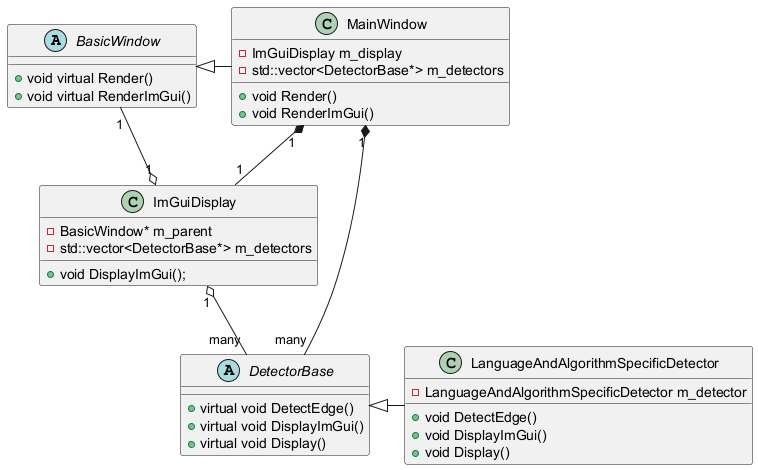
\includegraphics[width=0.8\linewidth]{view}
\caption{Class diagram of view plan}
\label{fig:class_view_plan}
\end{figure}

As we can see in \autoref{fig:class_view_plan} the plan was that I have a basic abstract window class named \textit{BasicWindow} in my own pipeline abstraction and implement a main window from that. Because of the complexity of the ImGui display I choose to use a class to abstract out the common elements. Lastly the detectors themselves are implementing a base class so I can store them in the main window but still have different implementation for all the algorithms in all the languages. This means that we would have 6 of these classes because of this as we will see later in \autoref{chap:Imp_Arc} this changed while developing and I will explain the reason for it in that subsection. As I have stated above there was no plan for the synthetic tester to have different class structure so the only difference is how the ImGui looks.

As for the models architecturally I use the two libraries that we are testing to implement the algorithms on the \ac{GPU} and I used no external libraries to implement the algorithm on the \ac{CPU}

\begin{figure}[H]
\centering
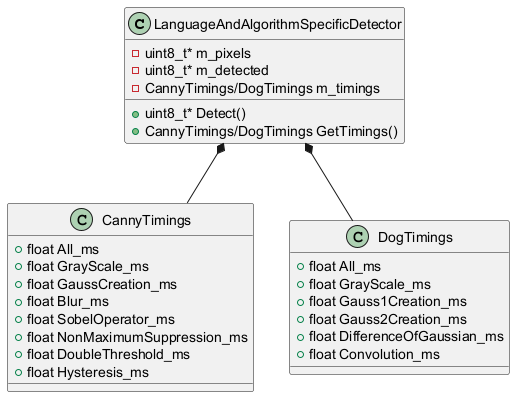
\includegraphics[width=0.8\linewidth]{model}
\caption{Class diagram of model plan}
\label{fig:class_model_plan}
\end{figure}

For the plan of the class structure because on CUDA we need separate functions, and for OpenCl we need separate kernel files, I thought that we cannot abstract out any common element except for the struct for the timings, I choose to just create separate classes for them. We can see this reflected on the Class diagram in \autoref{fig:class_model_plan} but as with the View as I started implementing it this planed changed slightly and we will discuss this latter at \autoref{chap:Imp_Arc}.

\subsection{Algorithms}
\label{chap:algo}

So far I only talked about my plans for the view and class structure but by an early stage I know which edge detection algorithms I want to implement and as we have already discussed it in \autoref{chap:intro} they are: \ac{Canny} and \ac{DoG}. In this subsection I will demonstrate my plan for the algorithms.

\subsubsection{Canny edge detection}

According to the original article\cite{canny:paper} the \ac{Canny} algorithm has 4 steps

\begin{enumerate}
\item Filter out any noise. The Gaussian filter is used for this purpose.
\item Find the intensity gradients of the image. For this purpose I use the Sobel filter.
\item Non-maximum suppression is applied. This removes pixels that are not considered to be part of an edge.
\item Hysteresis with double thresh holding. I choose to do this in two steps.
\end{enumerate}

The original article\cite{canny:paper} is very detailed but it's a hard read thus I used other sources\cite{canny:imp}\cite{canny:imp2} to understand the concept better and formulate the algorithms.

Firstly before we can do anything we have to grey scale the image. This is a very simple algorithm as we can see in algorithm \ref{alg:grey} we just take the RGB pixel values and multiply them by 0.2999, 0.587, 0.114 accordingly,

\begin{algorithm}[H]
\caption{Grey scaling algorithm}
\label{alg:grey}
\begin{algorithmic}
\State \textbf{Data:} $I$ the RGB pixels of the image
\State \textbf{Result:} $I2$ the grey scaled value of the pixels
\For{$r \; g \; b$ pixel values in $I$ image}
\State $p = 0.299 * r + 0.587 * g + 0.114 * b$
\State where $p$ is the pixel value cores ponding in $I2$
\EndFor
\end{algorithmic}
\end{algorithm}

Now we can focus on the edge detection algorithm properly first is the Gaussian blur. We could use other blurring methods but this is the simplest for our purpose and we can later reuse this in the \ac{DoG} algorithm.

\begin{algorithm}[H]
\caption{Gaussian blur}
\label{alg:gauss}
\begin{algorithmic}
\State \textbf{Data:} $I$ the grey pixels of the image, $G$ the values in the Gaussian kernel in a matrix, $k$ is the size of the kernel
\State \textbf{Result:} $I2$ the output value of the pixels
\For{$c,r$ where $c$ is the index for the column and $r$ is the index for the row of the pixel in $I$ image}
\State $s = 0$
\For{$i=-\frac{k-1}{2},\ldots,\frac{k-1}{2}$}
\For{$j=-\frac{k-1}{2},\ldots,\frac{k-1}{2}$}
\State $s = I[c + i ][r + j] * G[i][j] + s $
\EndFor
\EndFor
\State $I2[c][r] = s$
\EndFor
\end{algorithmic}
\end{algorithm}

In the next step we are going to calculate the intensity gradient and the edge direction for the image. This step is where we will final get edge lines before this we were only doing preliminary work. The gradient will be our edges and we can calculate the edge directions too which we will use in the next step when we do the Non-maximum suppression to find a single edge line. We use the 2 directionel 

\begin{algorithm}[H]
\caption{Intensity gradient}
\label{alg:sobel}
\begin{algorithmic}
\State \textbf{Data:} $I$ the pixels of the image
\State \textbf{Result:} $I2$ the intensity gradient value of the pixels, $I3$ is the edge direction of the pixels
\For{$c,r$ where $c$ is the index for the column and $r$ is the index for the row of the pixel in $I$ image}
\State $SX = \{-1, 0, +1, -2, 0, +2, -1, 0, +1\}$
\State $SY = \{+1, +2, +1, 0, 0, 0, -1, -2, -1\}$
\State $sx = 0$
\State $sy = 0$
\For{$i=-1,\ldots, 1$}
\For{$j=-1,\ldots, 1$}
\State $sx = I[c + i ][r + j] * SX[i][j] + sx $
\State $sy = I[c + i ][r + j] * SY[i][j] + sy $
\EndFor
\EndFor
\State $I2[c][r] = \sqrt{sx^2+sy^2}$
\State $t = \frac{\text{atan2}(sx,sy) * 180}{\pi} $
\If{$t < 180$}
\State $t = t + 180$
\EndIf
\State $I3[c][r] = t$
\EndFor
\end{algorithmic}
\end{algorithm}

Next comes the non maximum suppression in this step we will filter out the gradient so that only continuous edges remain for this purpose we will use the edge direction's we got from the previous step.

\begin{algorithm}[H]
\caption{Non-Maximum suppression}
\label{alg:max}
\begin{algorithmic}
\State \textbf{Data:} $I$ the intensity gradient of the image $I2$ the edge direction of the pixels 
\State \textbf{Result:} $I3$ the pixels of the image that only contain continuous edges
\For{$c,r$ where $c$ is the index for the column and $r$ is the index for the row of the pixel in $I$ image}
\State $q,r = 2000$
\If{$0 \leq I2[c][r] < 22.5$ or $157 \leq I2[c][r] \leq 180$}
\State $q = I[c][r + 1]$
\State $r = I[c][r - 1]$
\ElsIf{$22.5 \leq I2[c][r] < 67.5$}
\State $q = I[c + 1][r - 1]$
\State $r = I[c - 1][r + 1]$
\ElsIf{$67.5 \leq I2[c][r] < 112.5$}
\State $q = I[c + 1][r]$
\State $r = I[c - 1][r]$
\ElsIf{$112.5 \leq I2[c][r] < 157.5$}
\State $q = I[c - 1][r - 1]$
\State $r = I[c + 1][r + 1]$
\EndIf
\If{$I[c][r] \geq q$ and $I[c][r] \geq r$}
\State $I3[c][r] = I[c][r]$
\Else
\State $I3[c][r] = 0$
\EndIf
\EndFor
\end{algorithmic}
\end{algorithm}

The next step I choose to do separately into two separate because of the nature of the  algorithms but in reality they are just one the hysteresis. In the first step the double thresh holding where we categorize the edges into two groups weak edges and strong edges. Based on this then we take all the weak pixels and transform them into strong pixels only in the case when the week pixel have atleast one strong pixel sounding it.

\begin{algorithm}[H]
\caption{Double threshold}
\label{alg:thresh}
\begin{algorithmic}
\State \textbf{Data:} $I$ the pixels of the image, $l$ the low threshold, $h$ the high threshold
\State \textbf{Result:} $I2$ the week and strong pixels of the image
\For{$c,r$ where $c$ is the index for the column and $r$ is the index for the row of the pixel in $I$ image}
\If{$I[c][r] \geq h$}
\State $I2[c][r] = 255$
\ElsIf{$h > I[c][r] \geq l$}
\State $I2[c][r] = 125$
\Else
\State $I2[c][r] = 0$
\EndIf
\EndFor
\end{algorithmic}
\end{algorithm}

\begin{algorithm}[H]
\caption{Hysteresis}
\label{alg:hys}
\begin{algorithmic}
\State \textbf{Data:} $I$ the pixels of the image
\State \textbf{Result:} $I2$ the final image
\For{$c,r$ where $c$ is the index for the column and $r$ is the index for the row of the pixel where $I[c][r] = 125$}
\For{$i=-1,\ldots, 1$}
\For{$j=-1,\ldots, 1$}
\State $s =$ false
\If{$I[c + i][r + j] = 255 $}
\State $s$ = true
\EndIf
\EndFor
\EndFor
\If{$s =$ true}
\State $I[c][r] = 255$
\Else
\State $I[c][r] = 0$
\EndIf
\EndFor
\end{algorithmic}
\end{algorithm}

After we are done with the Hysteresis we are done with the algorithm and get our final picture.

\subsubsection{Difference of Gaussians}

This algorithm is much simpler then the previous while the \ac{Canny} have a lot of steps to get a fine tuned image it requires a per image fine tuning to get the best results. In comparison to that the \ac{DoG} algorithm requires much less fine toning but its less accurate too.

We basically already wrote the algorithm previously. First we use algorithm \ref{alg:grey} to gray scale the image. Than we only need algorithm \ref{alg:gauss} to use this. The only difference is that instead of supplying the algorithm a normal Gaussian kernel we first take the difference of two Gaussian kernels and we supply that kernel to the function. The resulting image will contain the edge lines of our image.

\section{Implementation}

\subsection{Architecture and Classes}
\label{chap:Imp_Arc}

\section{Testing}
\cleardoublepage
\chapter{Summary}

place holder
\cleardoublepage
\chapter*{Appendix}
\phantomsection
\addcontentsline{toc}{chapter}{Appendix}
\section*{List of Acronyms}
\phantomsection
\addcontentsline{toc}{section}{List of Acronyms}
\begin{acronym}
 \acro{GPGPU}{General-purpose computing on graphics processing unit}
 \acro{Canny}{Canny edge detector}
 \acro{DoG}{Difference of Gaussians}
 \acro{GPU}{Graphics processing unit}
 \acro{CPU}{Central processing unit}
 \acro{SDL2}{Simple Media Layer}
 \acro{ImGui}{Immediate mode graphics user interface library}
 \acro{ns}{Nano seconds}
\end{acronym}
\cleardoublepage

\phantomsection
\addcontentsline{toc}{section}{\lstfigurelabel}
\listoffigures
\cleardoublepage
\phantomsection
\addcontentsline{toc}{section}{\lstalgorithmlabel}
\listofalgorithms
\cleardoublepage
\phantomsection
\addcontentsline{toc}{section}{\biblabel}
\printbibliography[title=\biblabel]
\cleardoublepage
\end{document}